\begin{frame}[allowframebreaks]{Normalizing Flow Models}
    \begin{itemize}
        \item Consider a directed latent-variable model with observed variables $X$ and latent variables $Z$. In a normalizing flow model, the mapping between $Z$ and $X$ is deterministic and invertible: $G:\mathbb{R}^n \rightarrow \mathbb{R}^n$, such that $X=G(Z)$ and $Z=G^{-1}(X)$.
        \item By the change of variables formula, the marginal likelihood $p(x)$ is:
        $$
        p_X(x;\theta) = p_Z(G_\theta^{-1}(x)) \left| \det \left( \frac{\partial G_\theta^{-1}(x)}{\partial x} \right) \right|
        $$
    \end{itemize}
\framebreak

\begin{figure}
    \centering
    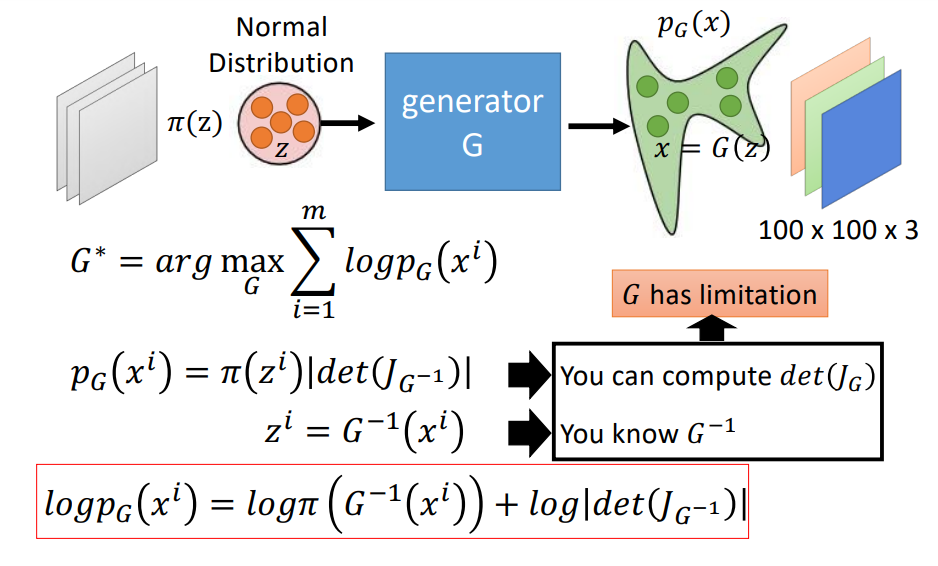
\includegraphics[height=0.9\textheight, width=\textwidth, keepaspectratio]{images/norm-flow/nfm_2.png}
\end{figure}

\framebreak

\begin{itemize}
    \item The expressiveness of $G$ is limited. To model more complex distributions, we need more expressive generators.
\end{itemize}

\begin{figure}
    \centering
    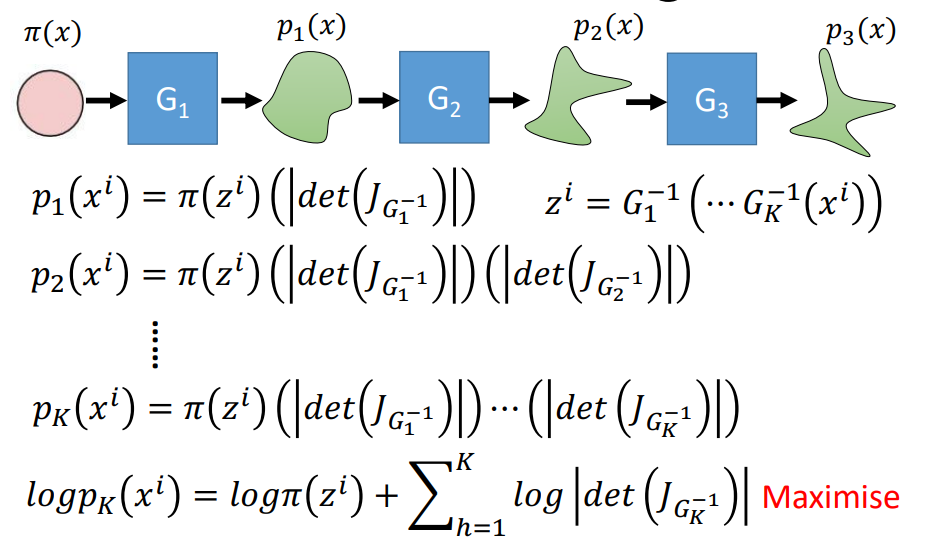
\includegraphics[height=0.9\textheight, width=\textwidth, keepaspectratio]{images/norm-flow/nfm_3.png}
\end{figure}

\framebreak

\begin{itemize}
    \item In practice, we train $G^{-1}$, but use $G$ for generation.
\end{itemize}

\begin{figure}
    \centering
    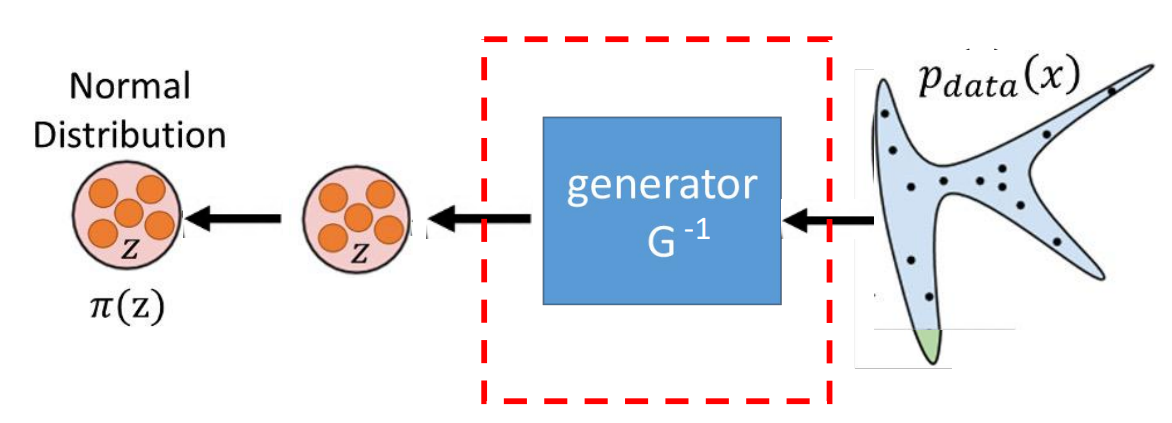
\includegraphics[height=0.5\textheight, width=\textwidth, keepaspectratio]{images/norm-flow/nfm_1.png}
\end{figure}

\framebreak

\begin{itemize}
    \item \textbf{Normalizing}: The change of variables produces a normalized density after applying an invertible transformation.
    \item \textbf{Flow}: Invertible transformations can be composed to create more complex, expressive mappings.
\end{itemize}
\end{frame}